\section{為什麼香港人在九七後才忽然熱衷爭取民主?}

香港人在九七前已經爭取民主。事實上,如果不是中國政府的阻撓,香港在九七前的民主進程可以走得更快。

英治時期香港的民主化,可由一九四六年的楊慕琦計劃說起。二次大戰結束,英國重新接管香港,總督楊慕琦提出香港推行自治。二戰後英國在世界各地的殖民地都有自治以至獨立運動,港英政府當時相信在香港推行自治可收籠絡民心之效,建議包括成立一個以直選議席為主的市議會,負責管理市政事務。不過,隨著國共內戰倒向共產黨的一方,中華人民共和國於一九四九年成立並於一九五零年與英國建交,中方向英方表明雖然不會急於收回香港,卻同時不會接受英方在香港推動民主,認為香港自治等於邁向獨立。於是乎,港英政府失去了政治改革的動機,及後三十年都沒有再推動,直到八十年代中英就香港前途問題談判才重新開始。有說香港的民主發展就像是「活化石」一樣,成為了英國最富庶卻同時是民主發展極為遲緩的屬地。

雖然如此,早期香港也有各式團體推動參政,例如香港革新會、香港華人革新會,和香港公民協會。與此同時,如前文所述,七十年代起香港本土意識開始形成,一批香港長大的年輕人熱心參與社會和為弱勢發聲,各式抗爭事件如中文運動、反貪污運動,和艇戶事件等為後來的民主運動殿下基礎。而為了回應六七暴動,政府也在同期開始鼓勵市民參與鄰里事務,例如清潔香港運動和撲滅罪行運動,並在公共屋邨組織互助委員會,成為公民參與的雛形。

到了八十年代,面對香港前途問題談判,培養香港人參與政治就變得更為重要。當時香港學界出現「民主回歸」的說法,即一方面否定英殖管治在香港的地位,同時認為中國收回香港是有條件的,特別是要對香港的民主發展有貢獻。近年有不少評論對這段歷史作出反思,認為當時的學界錯誤接受了中共的統戰,誤信中共管治下的「港人治港」可以糾正英殖封閉管治的問題,脫離了當時香港普遍不接受中共管治的主流意見。

無論如何,中英聯合聲明簽署後,為迎接九七後的「港人治港」,香港政制的民主化變得不能迴避。政府先於一九八一年發表《地方行政白皮書》,並於一九八二年開始區議會選舉。政府又於一九八四年發表《代議政制白皮書》,並於一九八五年首次進行立法局間接選舉。值得一提的是區議會剛成立的時候,香港民間曾有不同觀點。一些壓力團體不相信政府真的會開放參與,認為區議會只是另一種的「吸納政治」。不過也有另一派認為無論區議會本身有多少權力,席位本身所帶來的資源和公眾地位就很值得爭取,而選舉過程本身也可以成為動員公眾關心政治的手段。

% \begin{figure}[ht!]
%     \centering
%     \includemedia[
%     width=0.6\linewidth,height=0.45\linewidth,
%     activate=pageopen,
%     flashvars={
%         modestbranding=1  % no YT logo in control bar
%         &autohide=1       % controlbar autohide
%         &showinfo=0       % no title and other info before start
%     }
%     ]{}{https://youtu.be/3BJe2qpNvn4}   % Flash file
%     \caption{公民教育宣傳歌曲《蚌的啟示》1986 主唱:關正傑、區瑞強、盧冠廷}
% \end{figure}

% \begin{figure}[ht!]
%     \centering
%     \includemedia[
%     width=0.6\linewidth,height=0.45\linewidth,
%     activate=pageopen,
%     flashvars={
%         modestbranding=1  % no YT logo in control bar
%         &autohide=1       % controlbar autohide
%         &showinfo=0       % no title and other info before start
%     }
%     ]{}{https://youtu.be/rKQ_WZ31a9c}   % Flash file
%     \caption{公民教育宣傳歌曲《這區這裡》1988 主唱:張學友}
% \end{figure}

此外,市政局和區域市政局也為香港民主化作出過重要貢獻。市政局源於一八八三年成立的潔淨局,當時十名委員當中就有兩名由選舉產生。不過即使到了一九三五年改為市政局後,所謂的選舉仍然相當小眾,市民也不熱衷。當時規定必須要有一定教育、收入或專業程度的市民才可以成為選民,有估計到了一九七九年時仍只有四十四萬人合資格,即當時人口的十分之一;而這些人當中只有三萬五千人登記為選民,而在一九八一年的選舉中只有六千多人投票。不過到了市政局隨八十年代的代議政制發展而變得開放,也和區議會一樣成為培養政治人才的地方。一九八三年選出的市政局議員當中,既有元老人物如杜葉錫恩,也有當時的政界新星如譚惠珠、馮檢基和李植悅等。隨著新市鎮的發展,在新界負責相同功能的區域市政局也在一九八六年成立。

基層選舉的出現對香港的民主發展十分重要。殖民地早期的立法局完全由官方主導,後來通過委任非官守議員把商界菁英(包括華人領袖)來加強管治認授,也就是前文提過「行政吸納政治」的套路(見問題二十)。回到七十年代的立法局,主席由港督兼任,一半的議員由政府官員出任,另一半則由港督委任,換言之只有政府認可的人才能成為議員。到了一九八五年,立法局的組成改為官守議員十名,委任議員二十二名,功能界別議員十二名,以及由市政局、區域市政局和區議員互選產生的十二名選舉團議員。雖然官守議員和委任議員仍佔過半數,不過因為市政局、區域市政局和區議員本身已有直選產生的議員,所以選舉團的互選就間接成為一般市民晉身立法局的途徑(不過由於區議會等本身也有很多委任議員,加上相對接近官方的街坊組織,親政府的勢力在選舉團仍有優勢)。在一九八五到一九九一年期間,立法局內常有六、七名議員提出相對批判的意見,如司徒華和李柱銘等。當立法局有了反對的聲音,儘管只是少數,立法局的議事文化也隨之而改變,以前可以數小時內把法案三讀通過的運作模式變得過時,而傳媒對反對聲音的關注也成為一種面向整個社會的民主教育。

\begin{figure}[htbp]
    \centering
    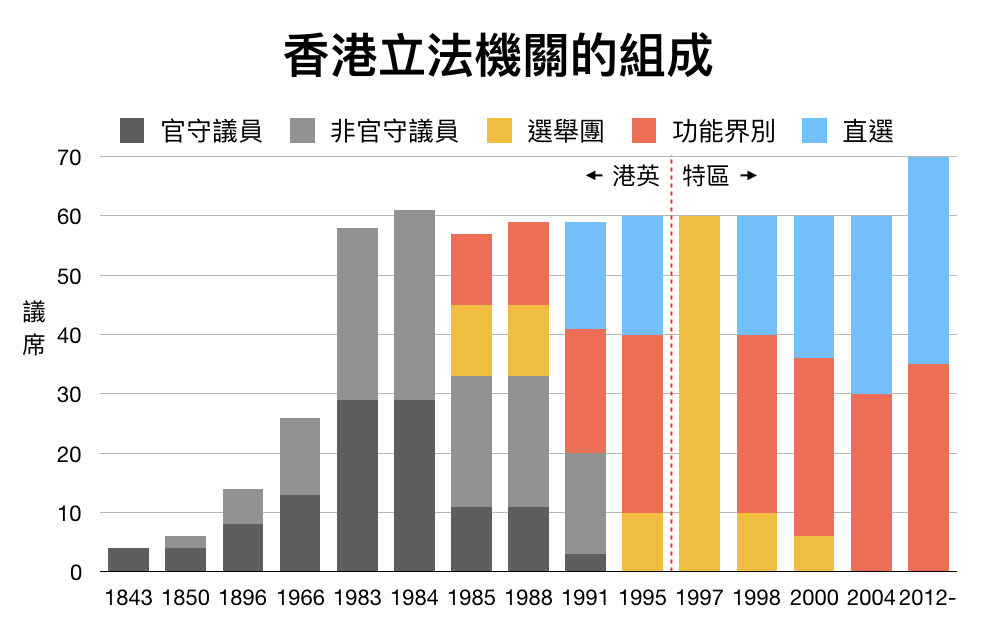
\includegraphics[width=0.7\textwidth]{c32/h-klesson1-051.png}
    \caption{圖香港立法機關的組成在九七前有快速的民主化,但九七後進展緩慢} 
\end{figure}

與此同時,香港民間也意識到民主化可以是回應「九七大限」的一種積極手段,也就是所謂「民主限共」或「民主抗共」的說法。注意當時的香港和今天的形勢十分不同,立法局還未有直選議席,民主選舉是一件十分新鮮的事情,社會對其潛力與限制尚在摸索之中。與此同時,中國大陸剛剛走出文革,號召改革開放,《基本法》則尚在草擬階段,所以當時不少意見領袖都視「民主限共」或「民主抗共」為合理的政治路線。

來到一九八六年,各民主派組織和社會團體於高山劇場舉行「高山大會」,討論《基本法》的起草和香港的政制法展,並成立了民主政制促進會。民促會的首個目標,是在一九八八年的立法局選舉當中引入直選議席。政府當時發表了《綠皮書:一九八七年代議政制發展檢討》,就一九八八立法局選舉引入直選諮詢公眾意見,民促會在維多利亞公園舉辦了萬人集會支持引入直選。儘管當時的民意普遍支持八八直選,政府公佈的諮詢結果卻稱反對意見較多。後來經學者分析,發現當時政府刻意扭曲處理收到的意見,來達至民意不支持直選的結論。

按後來解密的英方檔案和末代港督彭定康在其回憶錄內所述,是次扭曲民意之舉的背後是中方和英方的秘密協議。中方認為當時《基本法》尚在草擬階段,如果英方在期間落實在立法局推行直選,等於製造既定事實限制《基本法》的草擬。結果英方決定拒絕八八直選,換來中方保證把直選寫進《基本法》當中。

說到《基本法》於八十年代後期的草擬,香港各界已對當中的政制安排提出各種意見,足證香港人對香港民主的追求絕非九七後才忽然出現。而民促會推薦的「一九零直選方案」,當中的要求到今天仍然未能實現。所謂「一九零方案」,是指由一百九十名不同界別人士於一九八六年聯合提出的政制方案。他們要求立法機關不少於一半議席由一人一票直選產生,不少於四分之一由區議會構成的選舉團間接產生,不多於四分之一由功能界別產生。至於行政長官選舉,則由不少於十分之一的立法機關議員提名,全港市民一人一票直選產生。如果按照這個方案的話,香港在一九九七年七月一日特區成立的第一天,便應已有普選產生的行政長官。

基本法諮詢委員會沒有接受這個方案。當時獲接受的是「雙查方案」,即首三屆行政長官選舉由選舉團方式產生,也就是現時《基本法》所列的選舉委員會。不過,「雙查方案」和最終《基本法》的定稿有一個重要分別。按一九八九年一月通過的《基本法》草案第二稿,原有規定在第三任行政長官和第四屆立法會任內,舉行全民投票決定普選產生行政長官和全體立法會議員。這建議在當時已經被視為過於緩慢和保守,不過在經歷八九民運之後,到了一九九零年四月正式通過《基本法》時,就連規定全民投票的條文也不復見。

\begin{figure}[htbp]
    \centering
    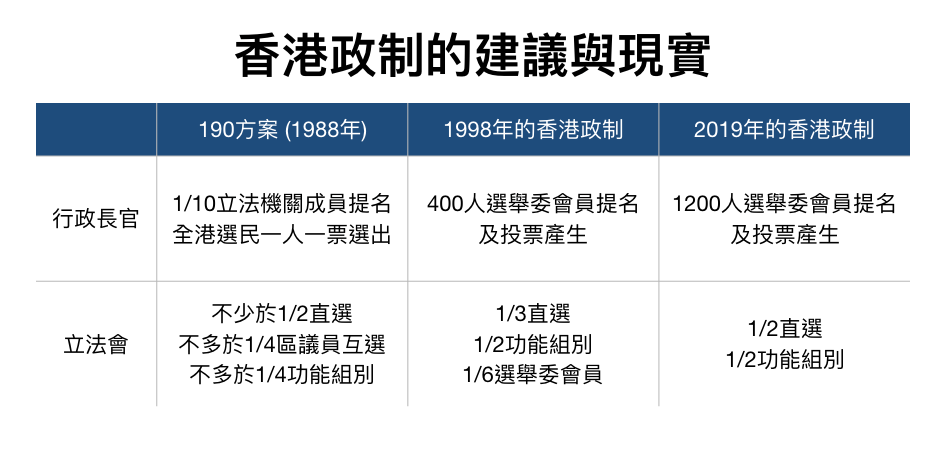
\includegraphics[width=0.7\textwidth]{c32/h-klesson1-052.png}
    \caption{今天香港政制的民主程度不如1988年的民間建議} 
\end{figure}

八九民運也為香港的民主化帶來另一影響:英方意識到有需要加快香港的民主化。由於《基本法》已規定特區的首屆立法會將會有二十席的直選議席,港英政府順理成章於一九九一年在立法局引入直選以作銜接。該屆選舉既為香港首次容許立法機關有議席由直選產生,加上距離八九民運只有兩年,於是民主派大獲全勝,十八席直選議席當中取得十四席。該屆選舉為雙議席雙票制,原來的估計選民會一票投給民主派,另一票投給其他候選人,結果選民卻大多把兩票都投給民主派(即「西瓜效應」)。隨著直選出現和民主派的勢力增加,立法局的運作模式進一步改變:內會不再是閉門會議、內會主席由議員互選產生、行政和立法分家、委員會制度常規化等等,逐漸增加了立法局的監督能力,甚至可以影響政策。例如由胡紅玉議員提出的反歧視法案雖然被否決,卻最終促使政府提出其版本的條例,並成立了平等機會委員會。

到了一九九五的立法局選舉,所有議席首次全數由選舉產生,而且民主成份按彭定康的政改方案大幅增加。新增的九個功能團體席位被設定成「變相直選」,而二十席直選則以單議席單票制選出,讓民主派得到很大優勢,結果選出香港歷史上唯一一次民主派佔多數的立法機關。不過,由於中方拒絕承認這次選舉,選出的議員無法案原定安排於一九九七年七月一日順利過渡成為首屆立法會的議員(見問題六),並由臨時立法會取代之。

儘管如此,這屆只有兩年任期的末代立法局仍然十分重要。首先,隨著官守和委任議員退場,立法局主席也不再由港督兼任。這屆立法局在有限任期內通過了不少重要的法例,特別是由議員自行提出的私人法案,例如禁止在維多利亞港填海的《保護海港條例》,以及給予工會法定談判權的《集體談判權條例》。在這兩年間,議員共提出了五十三條私人法案,當中二十六條獲得通過。

不過,《集體談判權條例》在一九九七年六月二十六日通過後,隨即於七月十六日被臨時立法會所凍結,並於十一月正式廢除。當年推動此法的職工盟秘書長李卓人稱《集體談判權條例》可能是全世界最短命的法例之一。除此之外,臨時立法會還推翻了很多過去的決定。例如《公安條例》對遊行集會的發牌制度原於一九九五年因牴觸《公民權利和政治權利國際公約》而被廢除,卻在一九九七年由臨時立法會重訂為今天的「不反對通知書」制度(見問題二十九)。而立法會地區直選的選舉方法本身,也從一九九一年的雙議席雙票制改為一九九五年的單議席單票制後,再於一九九八年改為比例代表制的最大餘額法,儘管當時民意調查顯示市民喜歡以個人而非政黨作為選擇基礎。比例代表制的最大餘額法結果在實踐中演變成多議席單票制,種下日後立法會政黨碎片化的根源(見問題二十二)。

總括來說,香港人對民主化的訴求並非九七後才忽然出現。事實上,隨著各社會和壓力團體在七十年代開始活躍,香港的民主化在九七前已有長足發展。而如果不是中方對香港民主化有所避諱的話,過渡期間的民主化進程甚至可以走得更快。而隨著臨時立法會的成立,香港的民主發展更有所倒退。

最後,若要衡量九七對香港人爭取民主的影響,則是香港人發現此事在九七後更有迫切。英治時代的香港雖然只有有限民主,但英國本身是一個民主國家,英國社會對法治和人權的重視也有悠久的歷史,並且隨之伸延至香港,例如香港政府廢除華人社會中的「妹仔」(蓄婢)制度,就可以從英國下議院的相關討論說起。此外,由於當時香港處於冷戰前沿,港英政府有意識要保持香港社會穩定,以免中共借機在港生事,所以即使沒有制度上的民主,但是港英政府仍然十分重視保持其管治認授。上述兩點都隨著九七來臨而消失,中國政府本身不是一個民主政府,管治制度與文化和香港格格不入;中國政府亦以為自己在香港的管治認授不證自明。如果者,不少香港人會感到民主制度在九七前可有可無,但到了九七後卻變得必不可少,因為香港的宏觀處境已不再一樣。他們發現,當香港沒有民主制度的話,就很難保障其他方面(如法治和人權)的制度穩健。

更重要的,是九七前的香港社會一直面臨「九七大限」,不少人把香港稱之為「借來的時間、借來的地方」,即使個人生活層面也是搵快錢至上,更別說要為整個香港的未來說得太遠。畢竟在港英之下爭取民主,也要面對九七後被全盤推翻的可能;然而到了九七之後,按照港人治港的原則,香港理應是「我們的時間、我們的地方」。香港人在九七後對香港政府的認授問題比九七前更為重視,只不過是要兌現中國政府本來的承諾,實屬正常不過。

伸延閱讀:

馬嶽(2010):《香港政治:發展歷程與核心課程》,香港:香港中文大學香港亞太研究所。

馬嶽(2012):《香港80年代民主運動口述歷史》,香港:香港城市大學出版社。

Sing M (2004) \textit{Hong Kong’s Tortuous Democratization: A Comparative Analysis}. New York: RoutledgeCurzon.

